\documentclass[conference]{IEEEtran}
\IEEEoverridecommandlockouts

\usepackage{cite}
\usepackage{amsmath,amssymb,amsfonts}
\usepackage{graphicx}
\usepackage{booktabs}
\usepackage{xcolor}
\usepackage{url}
\usepackage{tikz}
\usetikzlibrary{arrows.meta,positioning,calc,fit,backgrounds}
\usepackage[hidelinks]{hyperref}

\begin{document}

\title{An RF-Emergent MCS-Downgrade Reactive Jamming Attack on Industrial 5G
Link Adaptation}

\author{\IEEEauthorblockN{Author Name}
\IEEEauthorblockA{Affiliation \\
\texttt{email@example.com}}}

\maketitle

\begin{abstract}
Factories are starting to run their machine controls over private 5G networks, where
every message has to arrive on time. To stay fast, 5G keeps changing the speed of each
link based on how good the radio signal looks. It sets the speed with a value called a
Modulation and Coding Scheme (MCS), and it chooses the MCS from two feedback signals
sent back by the receiver. 5G protects neither signal against tampering. We show how an
attacker can abuse this. The attacker stays quiet until the link is running fast, then
sends a short burst of interference that spoils one block of data. The failed block
makes the network think the link has gone bad, so it lowers the speed. By repeating
this, the attacker keeps the link stuck at a low speed. Messages then take too long,
miss their deadlines, and the control loop breaks.

We build this attack in a 5G network simulator (ns-3 5G-LENA). In this simulator
interference builds up gradually and runs through a real error model, so a jammed block
is damaged but still received, not simply thrown away. We also add a common speed-control
feature that the simulator was missing, called outer-loop link adaptation (OLLA). With
these pieces in place the slowdown happens on its own, straight from the radio model,
with nothing faked: the link speed falls from near the top setting to near the bottom,
and only when the outer loop is turned on. This is our main result, and a simpler
simulator that just drops jammed blocks cannot show it. On a clear, direct radio path
the attack causes as many missed deadlines as ordinary always-on jamming while
transmitting only about a quarter of the time. We give this as a best case: on a
realistic, randomly changing channel the attack still works cheaply in most setups, but
fails when the attacker has no clear path to the victim. We also list the simplifying
assumptions behind the result.
\end{abstract}

\begin{IEEEkeywords}
industrial 5G, link adaptation, reactive jamming, MCS downgrade, OLLA, HARQ, URLLC,
ns-3, denial of service.
\end{IEEEkeywords}

\section{Introduction}
Factories are starting to run their machines over private 5G networks. These networks
carry the traffic of industrial control systems (ICS): the small, frequent messages
that programmable logic controllers (PLCs), sensors, and actuators exchange to run a
process. This traffic has hard timing limits. A message that arrives late can stall a
conveyor, overflow a tank, or trip a safety interlock~\cite{lenz2026security,
michaelides2025secure}. 5G offers a service class for exactly this need, called
ultra-reliable low-latency communication (URLLC). The timing budget is tight, so even
small protocol overheads matter~\cite{michaelides2026latency}.

We study an attack that turns one of 5G's main features against this promise. The
feature is \emph{link adaptation}: the network keeps choosing how fast to send data,
based on how good the channel looks (we explain it in Section~\ref{sec:bg}). The key
point is simple: when the network sees data fail to arrive, it slows the link down. An
attacker can make data fail on purpose, using short, well-timed bursts of interference,
and so push the speed down. A slower link means each control message takes longer to
send. If the attacker keeps the link slow, messages start missing their deadlines and
the control loop fails. We call this the \textbf{MCS-downgrade reactive jamming}
attack. The idea is not new in wireless generally: smart jamming can trap IEEE~802.11
rate adaptation at a low rate, because the link recovers more slowly than it backs
off~\cite{thapa2011rate}. Our contribution is to bring it to 5G link adaptation, make it
emerge from the radio model instead of injecting it by hand, and measure its impact on an
industrial control loop.

The whole attack rests on one step: a jammed fast block has to come back as a failure
report that the network then turns into a lower speed. This puts a requirement on any
simulator used to study it. The block has to be \emph{damaged but still received}, so
that it produces a failure report. If the simulator instead drops a jammed block before
its error model runs, the block just vanishes: no failure is reported, and the speed is
never lowered. Some industrial-5G testbeds model jamming in this all-or-nothing
way~\cite{lenz2026security}, and in such a model the attack cannot come out of the radio
layer by itself; someone must add it by hand.

We therefore build the attack in ns-3 5G-LENA, a 5G simulator where interference adds up
gradually. Every signal on the shared channel adds to the interference, the resulting
signal quality runs through a real error model, and a block can be damaged but still
received. Our contributions are:
\begin{enumerate}
\item We show that a steady interfering signal in 5G-LENA does not delete the victim's
blocks; it weakens them, so some arrive with errors. This is what the attack needs
(Section~\ref{sec:r1}).
\item We add the standard outer-loop (OLLA) feature to the 5G-LENA scheduler, which did
not have it, and apply its correction on every transmission
(Section~\ref{sec:bg}, Section~\ref{sec:methods}).
\item We build a jammer that watches the victim's link speed and jams only when it is
high. The speed then falls on its own, from the radio model, and only when the outer
loop is on (Section~\ref{sec:r2}).
\item We compare the attack with ordinary always-on jamming when the victim carries
time-critical traffic. On a clear radio path it causes the same number of missed
deadlines while transmitting only about a quarter of the time
(Section~\ref{sec:r3}); we give this as a best case, not a guarantee.
\item We test the attack on a realistic, randomly changing channel. It still works
cheaply in most setups, but fails when the attacker's path to the victim fades. We
report this as a result in its own right (Section~\ref{sec:r4}).
\item We check that the slowdown does not depend on how we tuned the outer loop: it
holds across a range of settings (Section~\ref{sec:r5}).
\end{enumerate}

\section{Background: How 5G Link Adaptation Works and Why We Attack It}
\label{sec:bg}

\subsection{Sending data: modulation and coding}
A 5G base station is called a gNB (next-generation NodeB). It serves user devices
called UEs (user equipment). We focus on the downlink (DL), the direction from the
gNB to the UE. The gNB sends data in units called transport blocks (TBs). For each TB
it picks a Modulation and Coding Scheme (MCS). The MCS sets how many bits the block
carries and how much error-correction it adds. A high MCS sends many bits in little
airtime but needs a clean channel. A low MCS sends fewer bits but survives a noisy
channel. In 5G the MCS is an index from 0 (lowest rate, most robust) to 28 (highest
rate). Choosing the MCS is a trade-off between speed and reliability.

\subsection{Choosing the MCS: two feedback loops}
The gNB cannot see the channel directly. It learns the channel from feedback, through
two loops (Fig.~\ref{fig:loop}).

The \emph{inner loop} uses the Channel Quality Indicator (CQI). The UE measures the
downlink quality, expressed as the signal-to-interference-plus-noise ratio (SINR), and
reports a CQI value. The gNB maps the CQI to an MCS that should keep the block error
rate (BLER, the fraction of blocks that fail to decode) near a target, often 10\%.

The \emph{outer loop} corrects the inner loop. After each block the UE sends Hybrid
Automatic Repeat reQuest (HARQ) feedback: an acknowledgement (ACK) if the block
decoded, or a negative acknowledgement (NACK) if it did not. A NACK on its own only
asks the gNB to resend the same block at the same MCS; it does not lower the rate. A
method called outer-loop link adaptation (OLLA)~\cite{sampath1997olla} adds that link. It keeps a small offset
per UE, lowers the offset on each NACK, and raises it on each ACK. The offset shifts the
chosen MCS until the real BLER matches the target. Without OLLA, only the CQI sets the
MCS, and decoding failures never lower it.

\begin{figure}[t]\centering
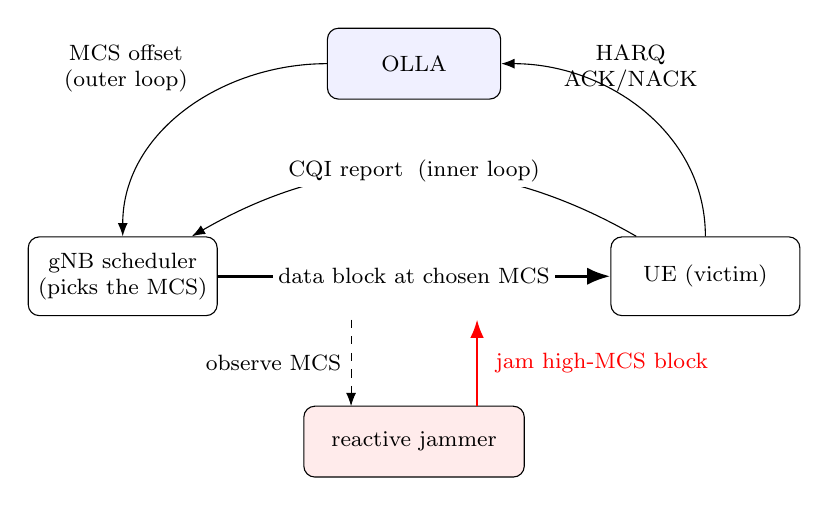
\begin{tikzpicture}[>=Latex,font=\footnotesize,
 box/.style={draw,rounded corners,align=center,minimum height=10mm,minimum width=24mm},
 olla/.style={draw,rounded corners,fill=blue!6,align=center,minimum height=9mm,minimum width=22mm},
 att/.style={draw,rounded corners,fill=red!8,align=center,minimum height=9mm,minimum width=28mm}]
 \node[box] (gnb) at (0,0) {gNB scheduler\\(picks the MCS)};
 \node[box] (ue)  at (7.4,0) {UE (victim)};
 \node[olla] (olla) at (3.7,2.7) {OLLA};
 % downlink data block (main path)
 \draw[->,very thick] (gnb) -- node[pos=0.5,fill=white,inner sep=2pt]{data block at chosen MCS} (ue);
 % INNER loop: CQI, small arc just above the data line (inside the outer loop)
 \draw[->] (ue) to[out=150,in=30]
   node[pos=0.5,fill=white,inner sep=1.5pt]{CQI report \;(inner loop)} (gnb);
 % OUTER loop: HARQ ACK/NACK up to OLLA, then MCS offset down to the scheduler
 \draw[->] (ue.north) to[out=90,in=0]
   node[pos=0.55,above,align=center]{HARQ\\ACK/NACK} (olla.east);
 \draw[->] (olla.west) to[out=180,in=90]
   node[pos=0.45,above left,align=center]{MCS offset\\(outer loop)} (gnb.north);
 % attacker below the data line
 \node[att] (j) at (3.7,-2.1) {reactive jammer};
 \draw[->,dashed] (2.9,-0.55) -- (2.9,-1.65) node[pos=0.5,left]{observe MCS};
 \draw[->,red,thick] (4.5,-1.65) -- (4.5,-0.55) node[pos=0.5,right=3pt]{jam high-MCS block};
\end{tikzpicture}
\caption{5G downlink link adaptation, and where the attacker acts. The gNB sends a data
block at the chosen MCS. Two feedback loops set that MCS: the \emph{inner loop} (the CQI
report, the small arc next to the data) and the \emph{outer loop} (HARQ ACK/NACK, which
feeds the OLLA correction back to the scheduler, the larger loop over the top). The
reactive jammer watches the victim's MCS and jams only high-MCS blocks; each jammed block
returns a NACK, which OLLA turns into a lower MCS.}
\label{fig:loop}\end{figure}

\subsection{Why this is a good target}
Two facts make link adaptation worth attacking.

First, the feedback is not protected. 5G does not integrity-protect CQI or HARQ at the
physical and link layers; this is part of a broader gap in the 5G control
plane~\cite{jover2019security}. An attacker cannot forge them, but it can change the channel
that produces them. A short, well-timed jamming pulse makes a high-MCS block fail to
decode. The UE then sends a genuine NACK. OLLA reads that NACK and lowers the MCS. The
attacker uses the network's own control loop against it.

Second, a low MCS breaks real-time control. Control messages are small and periodic
and have hard deadlines. A low MCS makes each message take longer to send. When the
link is trapped at a low MCS, messages miss their deadlines and the control loop
fails. The attacker does not need to block the link. It only needs to push the MCS
down and keep it there. This is cheaper and quieter than broadband jamming, which must
transmit all the time and is easy to detect~\cite{pelechrinis2011jammers}. We measure the attacker's cost as its duty
cycle: the fraction of time it actually transmits. A broadband jammer has a duty cycle
of one; a good reactive jammer has a much smaller one.

\section{Hypotheses and Methods}
\label{sec:methods}

\subsection{Threat model}
\label{sec:threat}
We state who the attacker is and what it may do, because the attack is built around
these limits, not around breaking them.

\textbf{Goal.} Deny availability of an industrial 5G link by trapping it at a low MCS,
so control messages miss their deadlines, while spending as little on-air time as
possible to stay cheap and hard to detect.

\textbf{What the attacker can do.} It is an outside party on the open air interface with
a jammer: a radio that can emit short bursts of interference on the victim's channel.
Reactive, sense-then-jam attacks like this run on commodity software-defined
radios~\cite{wilhelm2011reactive}. The attacker can also tell when the victim is using a
high MCS. In 5G the scheduling decision,
including the MCS, is carried in Downlink Control Information (DCI). The DCI is
\emph{scrambled} with the victim's identifier but is \emph{not} encrypted or
integrity-protected, so a passive receiver can decode it and read the MCS. This is not
hypothetical: open-source control-channel sniffers recover per-user DCI over the air on
commodity software-defined radios: in real time for LTE
(FALCON~\cite{falkenberg2019falcon}), and from live 5G NR networks
(5GSniffer~\cite{ludant2023sniffing}). The MCS and resource allocation are part of the DCI
those tools decode, so the information our jammer needs is obtainable in practice.
Obtaining it has two phases: \emph{locking} onto a specific victim's RNTI takes seconds of
exposure~\cite{ludant2023sniffing}, but once locked, each slot's MCS is read within about
one slot (FALCON does this in real time for LTE~\cite{falkenberg2019falcon}).

\textbf{What the attacker cannot do.} It cannot forge or inject feedback. The CQI and
HARQ ACK/NACK messages are scrambled, so the attacker cannot simply send a fake NACK to
push the MCS down. This is the key constraint: the attack must make the victim's own
device send a \emph{genuine} NACK, by corrupting a real block with interference. It works
one layer below the protocol, on the radio, so it never needs to read or write any
scrambled feedback message. The attacker also does not compromise the endpoints or have
physical access; those are out of scope.

\textbf{Idealizations in this study.} We assume the attacker has already locked onto the
victim and give the jammer the victim's MCS directly from the simulator, modelling only
the per-slot decode latency as an adjustable reaction delay; we do not model the
one-time, seconds-scale lock-on. This is an upper-bound (best-case) attacker. We make this and the
other simplifications explicit in Section~\ref{sec:validity}.

\subsection{Hypotheses}
We test three hypotheses.
\begin{itemize}
\item \textbf{H1.} In a graded-interference model, a constant interferer produces
received-but-corrupted blocks and real NACKs, not just dropped blocks.
\item \textbf{H2.} With OLLA on, a reactive MCS-aware jammer traps the victim at a low
MCS at a low duty cycle, and the downgrade is conditional on OLLA. The effect emerges
from the radio model, with no injected corruption.
\item \textbf{H3.} The reactive jammer reaches the same URLLC deadline-failure rate as
a broadband jammer at a much lower duty cycle.
\end{itemize}

\subsection{Simulator and scenario}
We use ns-3.47, an open-source discrete-event network simulator, with its 5G New Radio
(NR) module, called 5G-LENA, version~4.2~\cite{patriciello2019e2e}. Its physical-layer
abstraction maps SINR to block error rate using EESM curves calibrated against a
link-level simulator~\cite{lagen2020abstraction}, so co-channel interference produces
graded, measured errors rather than an all-or-nothing reception gate. The scenario has
two cells
(Fig.~\ref{fig:topo}). Cell~0 is the victim gNB and serves the victim UE at 20\,m.
Cell~1 is the interferer gNB and serves a second UE placed on top of the victim UE, so
its beam lands on the victim. Both cells share one 20\,MHz band at 3.5\,GHz. We use an
urban-microcell channel model with shadowing off, isotropic antenna elements, and
beamformed arrays. The victim cell transmits at 30\,dBm. We sweep or toggle the
interferer power.

\begin{figure}[t]\centering
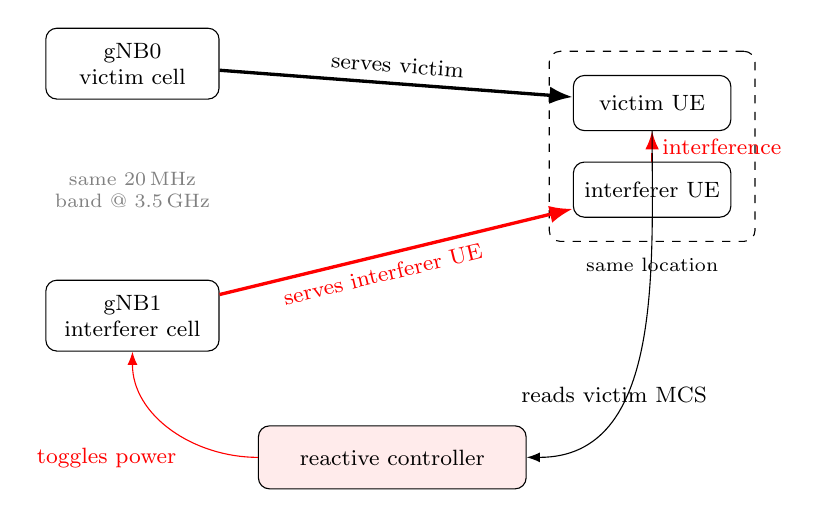
\begin{tikzpicture}[>=Latex,font=\footnotesize,
 gnb/.style={draw,rounded corners,align=center,minimum height=9mm,minimum width=22mm},
 ue/.style={draw,rounded corners,align=center,minimum height=7mm,minimum width=20mm},
 ctl/.style={draw,rounded corners,fill=red!8,align=center,minimum height=8mm,minimum width=34mm}]
 % left: two co-channel cells
 \node[gnb] (g0) at (0,1.6)  {gNB0\\victim cell};
 \node[gnb] (g1) at (0,-1.6) {gNB1\\interferer cell};
 % right: the two UEs sit at the same place
 \node[ue] (uv) at (6.6,1.1)  {victim UE};
 \node[ue] (uj) at (6.6,0.0)  {interferer UE};
 \begin{scope}[on background layer]
   \node[draw,dashed,rounded corners,fit=(uv)(uj),inner sep=3mm] (loc) {};
 \end{scope}
 \node[font=\scriptsize,align=center] at (6.6,-0.95) {same location};
 % serving links
 \draw[->,very thick] (g0) -- node[above,sloped]{serves victim} (uv);
 \draw[->,very thick,red] (g1) -- node[below,sloped,pos=0.45]{serves interferer UE} (uj);
 % because the interferer UE is on the victim, gNB1's signal IS the interference
 \draw[->,red,dashed,thick] (uj) -- node[right]{interference} (uv);
 % shared-channel annotation between the two cells
 \node[font=\scriptsize,align=center,gray] at (0,0) {same 20\,MHz\\band @ 3.5\,GHz};
 % reactive controller drives gNB1 from the victim's MCS
 \node[ctl] (c) at (3.3,-3.4) {reactive controller};
 \draw[->] (uv.south) to[out=-90,in=0] node[pos=0.7,above]{reads victim MCS} (c.east);
 \draw[->,red] (c.west) to[out=180,in=-90] node[pos=0.4,below left]{toggles power} (g1.south);
\end{tikzpicture}
\caption{How we realize the attacker of Fig.~\ref{fig:loop} in the simulator. The jammer
is built as a second cell (gNB1) on the \emph{same} 20\,MHz channel as the victim cell
(gNB0). gNB1 serves its own UE, which we place at the victim's location, so gNB1's signal
adds as interference on the victim. The reactive controller reads the victim's MCS and
switches gNB1's transmit power on and off. Compared with Fig.~\ref{fig:loop}, which shows
the mechanism, this shows the concrete radio setup that produces it.}
\label{fig:topo}\end{figure}

\subsection{OLLA loop}
5G-LENA selects the DL MCS from CQI alone; NACKs trigger only a same-MCS
retransmission. We add a standard OLLA loop. The idea is simple: nudge the rate down a
little on each failure and up a little on each success, so the failure rate settles at a
target. Each UE keeps an offset $\Delta$ in MCS-index units. On a DL NACK we set $\Delta \leftarrow \max(\Delta_{\min},
\Delta - s)$. On a DL ACK we set $\Delta \leftarrow \min(\Delta_{\max}, \Delta +
s\,B/(1-B))$, for step $s$ and target BLER $B$. We update $\Delta$ from freshly
received HARQ feedback only, so we never count a NACK awaiting retransmission twice. We
store the pure CQI-derived MCS as a base and re-derive the effective MCS,
$\mathrm{clamp}(\mathrm{round}(\mathrm{base}+\Delta),0,\mathrm{MCS}_{\max})$, at every
DL slot. This makes the offset act at HARQ speed, not only when a new CQI arrives. The
ACK step is smaller than the NACK step: at a 10\% target there are about nine ACKs per
NACK, and the factor $B/(1-B)$ balances them so the offset settles where the BLER equals
$B$. We use $s=0.1$ and $B=0.1$, and expose OLLA as an on/off switch.

\subsection{Reactive jammer}
The reactive jammer reads the victim's commanded DL MCS from the per-block trace and
controls the interferer power. While the observed MCS is at or above a threshold, it
sets the interferer to high power (jam). Below the threshold, it sets it to low power
(silent). It runs on a 100\,$\mu$s tick and reports its duty cycle (the fraction of
ticks spent jamming), which we use as the on-air cost. Reading the victim's MCS is a
realistic capability because the DCI is unprotected (Section~\ref{sec:threat}); here we
read it from the trace and discuss that idealization in Section~\ref{sec:validity}. We
use a threshold of 10.

\subsection{Traffic, plant, and metrics}
For link-adaptation measurements the victim runs saturating DL traffic (the link always
has data to send). For the impact study the victim runs periodic URLLC traffic: one
1000-byte packet every 1\,ms with a 2\,ms deadline.

To measure physical impact we attach a simple closed-loop process to the victim,
modelled on a bottle-filling plant. A remote controller sends one command per URLLC
packet. While commands arrive on time, the actuator holds a tank at its set level. If a
command is late, the inlet valve stays open and the tank fills; if enough commands are
missed in a row, the tank overflows and we count a fault (a safety event). This turns
link-level deadline misses into a physical-damage count.

We read the commanded MCS, the corrupt flag, and the BLER from the per-block trace. A
control packet is useful only if it arrives before its deadline, so we measure the
URLLC failure rate as the fraction of packets that are lost or late,
$(\mathrm{tx}-(\mathrm{rx}-\mathrm{late}))/\mathrm{tx}$, where \emph{late} packets
arrive after the deadline. This counts both lost and late packets and does not
undercount packets still queued at the end of the run. We report the jammer duty cycle
as the attacker cost. We run on the line-of-sight (LOS) channel to isolate the
mechanism from the random line-of-sight / non-line-of-sight (NLOS) draw. The channel is
random, so we repeat each case over several random seeds and report the spread as a
95\% confidence interval (CI), computed with the Student-$t$ distribution.

\section{Results}

\subsection{R1: Interference is graded, not all-or-nothing}
\label{sec:r1}
We sweep the constant interferer power and read the victim's DL blocks
(Table~\ref{tab:r1}). The number of received blocks stays at 1597 across all powers:
the blocks are received, not gated out. The SINR falls smoothly from 67.5\,dB to
$-8.6$\,dB. The corrupt fraction rises from 0 to 52.6\%. This is the
received-but-corrupted regime the attack needs, and it confirms H1. The MCS already
tracks down through CQI here; the NACK-driven downgrade is the next step.

\begin{table}[t]\centering
\caption{R1: victim DL blocks vs.\ constant interferer power (saturating traffic).}
\label{tab:r1}
\begin{tabular}{rrrrr}\toprule
Power (dBm) & rx blocks & SINR (dB) & mean MCS & corrupt \\\midrule
off & 1597 & 67.5 & 27.9 & 0.0\% \\
30  & 1597 & 12.9 & 18.2 & 2.5\% \\
40  & 1597 & 1.3  & 6.6  & 3.8\% \\
50  & 1597 & $-8.6$ & 0.9 & 52.6\% \\\bottomrule
\end{tabular}\end{table}

\subsection{R2: The downgrade emerges from the radio model}
\label{sec:r2}
We first check the OLLA loop (Table~\ref{tab:r2a}). On a clean channel, OLLA on and
off give the same MCS (27.95) with no corruption, so the loop does not harm a good
link. Under constant 40\,dBm interference, OLLA raises the corrupt fraction from 3.8\%
to 9.3\%, close to the 10\% target: the loop reaches its set point. Here OLLA raises
the MCS, because constant interference also lowers the CQI, so the CQI-based MCS is too
cautious. The downgrade needs the opposite case: NACKs above target while the CQI
stays high. Selective jamming gives exactly that.

\begin{table}[t]\centering
\caption{R2: OLLA check, victim DL (saturating traffic).}
\label{tab:r2a}
\begin{tabular}{llrr}\toprule
Channel & OLLA & mean MCS & BLER \\\midrule
clean & off & 27.95 & 0.000 \\
clean & on  & 27.95 & 0.000 \\
jam 40\,dBm & off & 6.59 & 0.038 \\
jam 40\,dBm & on  & 8.62 & 0.093 \\\bottomrule
\end{tabular}\end{table}

We then run the reactive jammer (Table~\ref{tab:r2b}, Fig.~\ref{fig:mcs}). With OLLA
off, the jammer cannot trap the MCS. It runs 52\% of the time and the MCS stays near
14.6: the corrupted blocks only trigger same-MCS retransmissions. With OLLA on, the
NACKs drive the MCS down to 8.7, the jammer falls silent once the MCS drops, and its
duty cycle falls to 0.19. The downgrade is conditional on OLLA, and it emerges from
the radio model with no injected effect. This confirms H2.

\begin{table}[t]\centering
\caption{R2: reactive jammer, victim DL (LOS, threshold 10).}
\label{tab:r2b}
\begin{tabular}{lrrr}\toprule
OLLA & duty & mean MCS & corrupt \\\midrule
off & 0.52 & 14.6 & 43.4\% \\
on  & \textbf{0.19} & \textbf{8.7} & 17.4\% \\\bottomrule
\end{tabular}\end{table}

\begin{figure}[t]\centering
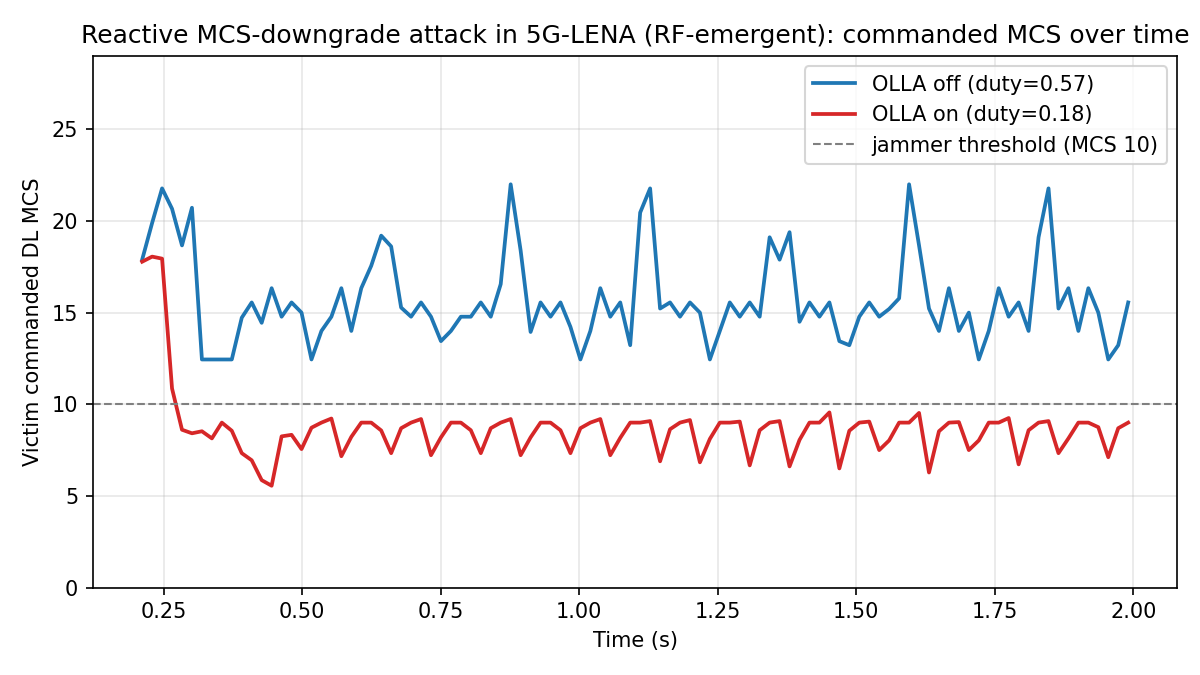
\includegraphics[width=\columnwidth]{paper-figs/commanded-mcs-5glena-reactive.png}
\caption{R2: victim commanded DL MCS over time under the reactive jammer. With OLLA
on the MCS collapses toward the threshold and stays trapped. With OLLA off it does
not.}
\label{fig:mcs}\end{figure}

\subsection{R3: Reactive jamming is cheaper than broadband}
\label{sec:r3}
We compare the reactive jammer against a broadband jammer (constant 40\,dBm, duty 1.0)
under URLLC traffic (Table~\ref{tab:r3}, Fig.~\ref{fig:tradeoff}). Both reach about
99.9\% deadline failure. The reactive jammer does so at a duty cycle of 0.255, against
the broadband jammer's 1.0: it reaches the same damage at about one quarter of the
on-air time. This confirms H3. The effect again needs OLLA: with OLLA off the reactive
jammer reaches the same failure rate but at a duty cycle of 0.611, so OLLA makes the
attack about $2.4\times$ cheaper. The confidence intervals on duty cycle do not
overlap.

\begin{table}[t]\centering
\caption{R3: URLLC impact vs.\ attacker cost (LOS, mean $\pm$ 95\% CI).}
\label{tab:r3}
\begin{tabular}{lrr}\toprule
Scenario & duty & failed\% \\\midrule
baseline & 0 & 0.2 \\
broadband 40\,dBm & 1.0 & $100\pm0$ \\
reactive, OLLA on & $0.255\pm0.080$ & $99.9$ \\
reactive, OLLA off & $0.611\pm0.020$ & $99.9$ \\\bottomrule
\end{tabular}\end{table}

\begin{figure}[t]\centering
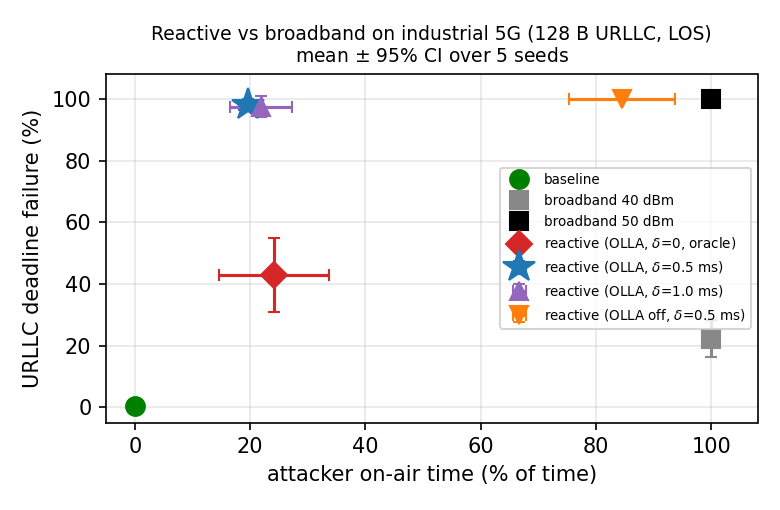
\includegraphics[width=\columnwidth]{paper-figs/tradeoff-ci-5glena.png}
\caption{R3: URLLC deadline failure vs.\ jammer duty cycle (LOS, 95\% CI over seeds).
The reactive jammer reaches the same failure rate as broadband at a far lower duty
cycle.}
\label{fig:tradeoff}\end{figure}

\subsection{R4: Under a realistic channel the attack is bimodal}
\label{sec:r4}
The efficiency figure in R3 is conditioned on a line-of-sight (LOS) channel, which we
use to isolate the link-adaptation mechanism from the random radio path. We now drop
that condition and run the standard random LOS/NLOS channel over many seeds
(Fig.~\ref{fig:regime}). The attack is \emph{bimodal}. On most realizations it works as
in R3: it traps the victim at a low duty cycle and drives URLLC failure to about 99.9\%.
On the rest, the jammer-to-victim path draws an NLOS fade; the jammer cannot reach the
victim, its controller never sees the MCS fall, its duty cycle runs to 1.0, and the
victim is spared. We report this as a result in its own right, not a footnote to R3: a
deployed attacker's success depends on the geometry of its own path to the victim.

Crucially the comparison is fair. The broadband jammer is channel-dependent too: its
mean failure rate falls from 100\% under LOS to 76\% under the random channel. The
baseline is invariant (0.2\% failure, no faults, every seed): all the variance lives on
the jammer-to-victim path, not the victim's own link. Conditioning on LOS therefore
removes a source of variance that weakens \emph{both} attackers, rather than favoring
ours. The defender takeaway is concrete: deny the attacker an LOS path to the victim.

\begin{figure}[t]\centering
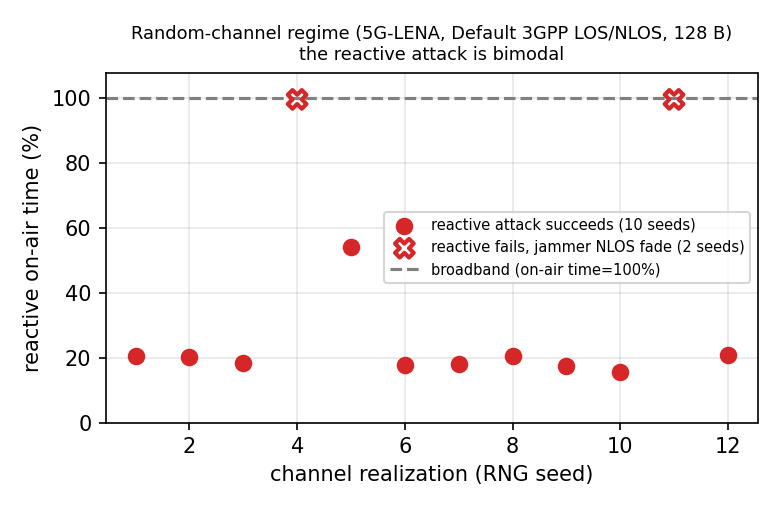
\includegraphics[width=\columnwidth]{paper-figs/channel-regime-5glena.png}
\caption{R4: reactive jammer duty cycle per channel realization (random LOS/NLOS). The
attack succeeds at a low duty cycle on most seeds and fails (duty $\to 1.0$) when the
jammer link draws an NLOS fade.}
\label{fig:regime}\end{figure}

\subsection{R5: The downgrade is robust to the OLLA tuning}
\label{sec:r5}
The attack exploits an OLLA loop we added, so we test whether the result depends on how
that loop is tuned. We sweep the OLLA step $s$ and target BLER $B$ over the reactive
attack (saturating traffic, LOS, three seeds each) and read the trapped MCS and the
jammer duty (Table~\ref{tab:r5a}). Across every one of the nine tunings the victim is
trapped between MCS~8.2 and~9.3, far below the OLLA-off mean of 14.9, and the jammer duty
stays between 0.14 and 0.38, always below the OLLA-off cost of 0.53. The downgrade is
therefore a property of the outer loop itself, not of the $s=0.1$, $B=0.1$ point used
elsewhere. The tuning shifts the operating point in the expected direction: a higher
target BLER tolerates more failures, so the jammer must fire more often (higher duty). It
never removes the trap.

\begin{table}[t]\centering
\caption{R5: trapped MCS and jammer duty vs.\ OLLA tuning (reactive, saturating, LOS,
mean over seeds). The trap holds for every tuning.}
\label{tab:r5a}
\begin{tabular}{llrr}\toprule
OLLA step $s$ & target $B$ & mean MCS & duty \\\midrule
\multicolumn{2}{l}{OLLA off (reference)} & 14.9 & 0.53 \\
0.05 & 0.05 & 9.3 & 0.20 \\
0.05 & 0.10 & 9.2 & 0.25 \\
0.05 & 0.20 & 9.3 & 0.38 \\
0.10 & 0.05 & 8.8 & 0.14 \\
0.10 & 0.10 & 8.8 & 0.20 \\
0.10 & 0.20 & 8.7 & 0.31 \\
0.20 & 0.05 & 8.6 & 0.14 \\
0.20 & 0.10 & 8.4 & 0.23 \\
0.20 & 0.20 & 8.2 & 0.38 \\\bottomrule
\end{tabular}\end{table}

We also re-run the sensing-delay sweep of the plant under three OLLA steps to test
whether the feedback resonance is an artifact of one tuning (Table~\ref{tab:r5b}). It is
not. For every step the per-packet failure rate stays pinned near 99.9\%, while the plant
fault count is non-monotonic in the delay with the same shape: low near zero delay,
high at 0.5--1.0\,ms, low again near 1.5\,ms, and saturated at 2.0\,ms. The resonance is
a structural property of the jammer--HARQ--plant loop, independent of the OLLA step.

\begin{table}[t]\centering
\caption{R5: mean plant faults vs.\ sensing delay for three OLLA steps (reactive,
URLLC+plant, LOS). Per-packet failure stays $\approx$99.9\% throughout; faults are
non-monotonic with the same shape at every step.}
\label{tab:r5b}
\begin{tabular}{rrrr}\toprule
delay (ms) & $s{=}0.05$ & $s{=}0.10$ & $s{=}0.20$ \\\midrule
0.0 & 88  & 50  & 45  \\
0.5 & 142 & 154 & 121 \\
1.0 & 158 & 152 & 156 \\
1.5 & 57  & 34  & 77  \\
2.0 & 170 & 170 & 170 \\\bottomrule
\end{tabular}\end{table}

\section{Analysis}
The results point to one load-bearing mechanism: the path from NACK to OLLA to MCS.
Graded interference (R1) supplies the corrupted blocks, but corruption alone does not
move the MCS. With OLLA off, the same corruption only triggers retransmissions
(R2--R3). The downgrade appears only when OLLA reads the NACKs and lowers the offset.
This is why the attack is cheap. The jammer does not block the channel; it steers the
adaptation loop and then waits. Once the victim is trapped at a low MCS, the jammer
can stay silent and the low MCS holds. A broadband jammer must transmit all the time
to cause the same damage.

Two further effects are worth noting.

\textbf{Sensing delay and a feedback resonance.} The damage to the closed-loop plant
of Section~\ref{sec:methods} is not a simple function of how often the jammer fires. We
vary the attacker's sensing delay (Fig.~\ref{fig:resonance}). The per-packet failure rate stays
near 99.9\% at every delay, but the number of faults changes by a large factor and is
not monotonic. Some delays cause few faults; others nearly saturate the count. The
reason is that a fault needs a run of consecutive misses, not just a high average miss
rate: the tank overflows only if the valve stays open long enough. So the same 99.9\%
per-packet failure can produce very different fault counts, depending on how the misses
cluster in time. At some delays the jammer fires through the victim's recovery windows,
so misses become contiguous and the actuator runs open for long stretches. This is a feedback resonance
between the jammer, the link-adaptation loop, and the control loop. The underlying
asymmetry is that the link recovers to a high MCS more slowly than the jammer pushes it
down. Smart jamming exploits the same asymmetry against Wi-Fi rate
adaptation~\cite{thapa2011rate}. So an attacker that tunes its reaction delay can raise
physical damage at the same on-air cost. The resonance is not an artifact of the OLLA tuning: it keeps the same shape across
OLLA step sizes (R5, Section~\ref{sec:r5}). It deserves separate study.

\begin{figure}[t]\centering
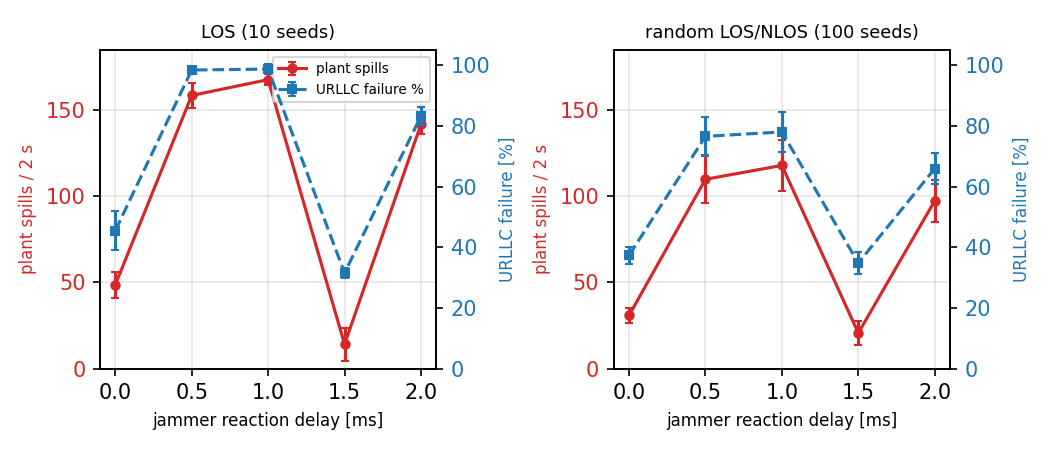
\includegraphics[width=\columnwidth]{paper-figs/delay-resonance-5glena.png}
\caption{Plant faults and per-packet failure vs.\ the attacker's sensing delay (LOS,
95\% CI over seeds). The per-packet failure rate stays saturated, but physical damage
is non-monotonic in the delay.}
\label{fig:resonance}\end{figure}

\textbf{Channel condition.} The efficiency figure is LOS-conditioned, and on the random
channel the attack is bimodal (R4, Section~\ref{sec:r4}). The variance sits on the
jammer-to-victim path, not the victim's own link, so the LOS condition does not favor our
attack.

\subsection{Threats to validity}
\label{sec:validity}
Our result is an existence proof in a system-level model, and three idealizations bound
how far the numbers carry to a real deployment. For each we state the direction of bias.

\textbf{The interferer is a rogue cell, not a jammer.} We produce graded interference
with a co-channel gNB that serves a co-located UE, so its beam lands on the victim. This
lets the interference flow through the simulator's native error model without a custom
physical layer, but the interfering waveform is a beamformed 5G NR signal, not jammer
noise. Its power and duty cycle are a cell's, not a real jammer's, and the exact
probability that one pulse fails one high-MCS block depends on a real jammer's waveform
and timing, which this model does not capture. Direction of bias: structured, perfectly
co-channel interference is favorable to the attacker, so a real jammer may need more
energy (higher duty) for the same effect. The atomic assumption (a short pulse fails a
high-MCS block) is the one we flag for link-level checking
(Section~\ref{sec:future}).

\textbf{The attacker reads the MCS through an oracle, not by decoding the DCI.} The
controller reads the victim's commanded MCS straight from the simulator trace and reacts
on a 100\,$\mu$s tick. In reality the MCS travels in the Downlink Control Information
(DCI), whose CRC is scrambled with the victim's identifier (RNTI) but is not encrypted or
integrity-protected. Reading it is therefore not just possible in principle but
demonstrated: real-time over-the-air DCI sniffers exist for LTE~\cite{falkenberg2019falcon}
and 5G NR~\cite{ludant2023sniffing}. What we do \emph{not} model is the decode itself; we
assume it succeeds and hand the jammer the value, with an optional reaction delay. Two
real-world costs are thus abstracted away. First is \emph{acquisition}: a 5G NR sniffer
must find the victim's RNTI and the PDCCH scrambling identity, which are configured over
encrypted signalling, so it blind-searches for them~\cite{ludant2023sniffing}. This is a
one-time, seconds-scale lock-on; the 5GSniffer experiments need seconds of exposure to
identify an RNTI. We assume the victim is already locked. Second is
\emph{per-decision latency}: once locked, the sniffer must read each slot's MCS within
about one transmission interval (roughly 0.5\,ms at our numerology; FALCON sustains this
for LTE's 1\,ms subframe~\cite{falkenberg2019falcon}). This staleness is what our
reaction-delay sweep covers, and the per-packet attack stays effective across it
(Section~\ref{sec:r5}), so a real decoder's latency sits inside the range we tested. One
caveat: the 5GSniffer evaluation decodes offline, not in real time, so the real-time
figure rests on FALCON and the one-interval bound, not on a measured NR number. We
therefore treat this as an \emph{upper-bound attacker}. This is a separate claim
from the integrity argument: the attack never forges feedback
(Section~\ref{sec:threat}); it only \emph{reads} unprotected control info to time its
pulses. Direction of bias: favorable to the attacker; the mechanism (NACK-to-MCS
coupling) is unchanged, only the efficiency figure would worsen.

\textbf{We exploit an OLLA loop we added ourselves.} 5G-LENA has no OLLA, so we ported a
standard one. Real gNBs run OLLA, so this is faithful in kind, but the attack's
exploitability depends on our step size and target error rate, which risks circularity.
We address this directly in R5 (Section~\ref{sec:r5}): the downgrade holds across a range
of OLLA tunings, so it is a property of the outer loop, not of one parameter set.

Two further limits are quantitative, not structural. The physical-process model is a
simple bottle-filling analog; its fault count tracks the \emph{clustering} of deadline
misses rather than their average rate, so it illustrates physical impact but is not a
calibrated plant. And our confidence intervals are over a small number of seeds; they
bound the spread within one geometry, not across deployments. None of these change the
central claim, which is qualitative: an RF-emergent, OLLA-conditional downgrade exists.

\section{Conclusion}
We built the MCS-downgrade reactive jamming attack in a higher-fidelity 5G simulator.
Because 5G-LENA models interference as a graded penalty and feeds it to a measured
error model, a jammed block is received-but-corrupted and produces a real NACK. We
added an OLLA loop, which the simulator lacks, and applied its offset at every DL slot.
The downgrade then emerged from the radio model with no injected effect: the victim
MCS fell from about 28 to about 9, and only when OLLA was on. This existence proof is
the central result, and it survives the OLLA tuning. On a line-of-sight path the attack
reached the same URLLC deadline-failure rate as broadband jamming at about one quarter of
the on-air time; we report this efficiency as a best case, because under a realistic
random channel the attack is bimodal: cheap and effective when the jammer can reach
the victim, defeated when it cannot. The attack is real in this model, it depends on
OLLA, and its cost depends on the attacker's path to the victim.

\section{Future Work}
\label{sec:future}

\textbf{Validate the per-block assumption at the link level.} Our system-level model
takes for granted the one physical-layer step the whole attack rests on: that a short,
low-energy interference pulse makes a high-MCS transport block fail its decode. A
link-level simulator can check this directly and cheaply, without the rogue-cell proxy.
The cross-check we plan uses NVIDIA Sionna (a GPU-based, 3GPP-compliant physical-layer
library; MATLAB's 5G Toolbox is an equivalent choice). For each MCS we encode a transport
block with the 5G NR low-density parity-check (LDPC) chain, pass it through a fading
channel, and measure the block error rate as a function of signal-to-interference ratio
under two interference shapes: continuous noise (the broadband baseline) and a short
pulse covering only part of the slot's symbols (the reactive attacker). The figure is a
family of BLER-vs-SIR curves, one per MCS, for each interference shape. It answers the
quantitative question our model cannot: how much energy, and over how few symbols, a
pulse needs to push a given high MCS past its decoding cliff. If the pulse curves sit
close to the continuous-noise curves at equal energy, the physical layer confirms the
efficiency claim; if they sit well above, the duty cycles are too optimistic and we
should rescale them. This turns the weakest assumption
(Section~\ref{sec:validity}) into a measured input.

\textbf{Defenses.} We did not test defenses. Three are worth measuring. An MCS floor for the URLLC slice
would cap the downgrade, at some cost to spectral efficiency. OLLA hardening, such as a
slower recovery or a bounded offset, would slow the trap. An anomaly detector could
flag NACK spikes that do not match the measured interference floor, or a fast MCS
collapse; the attack's low duty cycle and the feedback resonance are useful detection
signals. Beyond defenses, future work should test the attack over more geometries and
channels, validate it in a shielded lab with software-defined radios (SDRs), and couple
it to a higher-fidelity physical process.

\section*{Acknowledgments}
[Acknowledgments placeholder.]

\begin{thebibliography}{10}
\bibitem{patriciello2019e2e}
N.~Patriciello, S.~Lagen, B.~Bojovic, and L.~Giupponi,
``An E2E simulator for 5G NR networks,''
\emph{Simulation Modelling Practice and Theory}, vol.~96, p.~101933, 2019.

\bibitem{michaelides2025secure}
S.~Michaelides, S.~Lenz, T.~Vogt, and M.~Henze,
``Secure integration of 5G in industrial networks: State of the art, challenges and opportunities,''
\emph{Future Generation Computer Systems}, vol.~166, p.~107645, 2025.

\bibitem{michaelides2026latency}
S.~Michaelides, J.~Lapawa, D.~Eguiguren~Chavez, and M.~Henze,
``Evaluation of Security-Induced Latency on 5G RAN Interfaces and User Plane Communication,''
in \emph{Proc.\ 19th ACM Conf.\ on Security and Privacy in Wireless and Mobile Networks (WiSec '26)},
Saarbr\"ucken, Germany, 2026.

\bibitem{lenz2026security}
S.~Lenz, S.~Michaelides, M.~Rickert, J.~Holtwick, and M.~Henze,
``Security Implications of 5G Communication in Industrial Systems,''
in \emph{Proc.\ 11th ACM Cyber-Physical System Security Workshop (CPSS '26)},
Bangalore, India, 2026.

\bibitem{ludant2023sniffing}
N.~Ludant, P.~Robyns, and G.~Noubir,
``From 5G sniffing to harvesting leakages of privacy-preserving messengers,''
in \emph{Proc.\ IEEE Symp.\ on Security and Privacy (S\&P)}, 2023.

\bibitem{falkenberg2019falcon}
R.~Falkenberg and C.~Wietfeld,
``FALCON: An accurate real-time monitor for client-based mobile network data analytics,''
in \emph{Proc.\ IEEE Global Communications Conf.\ (GLOBECOM)}, 2019.

\bibitem{thapa2011rate}
B.~Thapa, G.~Noubir, R.~Rajaraman, and B.~Sheng,
``On the robustness of IEEE 802.11 rate adaptation algorithms against smart jamming,''
in \emph{Proc.\ 4th ACM Conf.\ on Wireless Network Security (WiSec)}, 2011.

\bibitem{wilhelm2011reactive}
M.~Wilhelm, I.~Martinovic, J.~B.~Schmitt, and V.~Lenders,
``Short paper: Reactive jamming in wireless networks: how realistic is the threat?,''
in \emph{Proc.\ 4th ACM Conf.\ on Wireless Network Security (WiSec)}, 2011.

\bibitem{pelechrinis2011jammers}
K.~Pelechrinis, M.~Iliofotou, and S.~V.~Krishnamurthy,
``Denial of service attacks in wireless networks: The case of jammers,''
\emph{IEEE Commun.\ Surveys Tuts.}, vol.~13, no.~2, pp.~245--257, 2011.

\bibitem{sampath1997olla}
A.~Sampath, P.~S.~Kumar, and J.~M.~Holtzman,
``On setting reverse link target SIR in a CDMA system,''
in \emph{Proc.\ IEEE 47th Vehicular Technology Conf.\ (VTC)}, 1997, pp.~929--933.

\bibitem{jover2019security}
R.~P.~Jover and V.~Marojevic,
``Security and protocol exploit analysis of the 5G specifications,''
\emph{IEEE Access}, vol.~7, pp.~24956--24963, 2019.

\bibitem{lagen2020abstraction}
S.~Lagen, K.~Wanuga, H.~Elkotby, S.~Goyal, N.~Patriciello, and L.~Giupponi,
``New radio physical layer abstraction for system-level simulations of 5G networks,''
in \emph{Proc.\ IEEE Int.\ Conf.\ on Communications (ICC)}, 2020.
\end{thebibliography}

\end{document}
